\chapter[Forschungsfrage 1]{Wie können Container-Anwendungen den Prozess des automatisierten \enquote{Deployments} unterstützen?} \label{ff1}
Dieses Kapitel ...

\section{Grundlagen: Definieren der Begrifflichkeiten zur Forschungsfrage eins}
Dieses Teilkapitel soll grundlegende Begrifflichkeiten, die im weiteren Verlauf dieser Arbeit verwendet werden, definieren, um so eine einheitliche Terminologie der Begriffe zu entwickeln. Dadurch wird ein gemeinsames Verständnis erzeugt.

\subsection{Methodik der Anforderungsanalyse}
Die Anforderungsanalyse leitet sich aus dem thematischen Komplex des \enquote{Requirements-Engineering} ab, die verschiedene Bedeutungsvarianten besitzt -- dabei \enquote{[...] steht [es] einmal für alle konkreten Aktivitäten am Beginn einer Systementwicklung, die auf eine Präzisierung der Problemstellung abzielen. Ebenso steht es aber auch für eine ganze Teildisziplin im Grenzbereich zwischen Systems-Engineering, Informatik und Anwendungswissenschaften.}\autocite[][S.19]{partsch_requirements-engineering_2010} Diese Analyse soll, laut der herrschenden Meinung der Wissenschaft, am Anfang jeder Systementwicklung stehen, um so bestimmte Vorgehensweise anzuwenden. Dabei entstehen, wenn der später weiter definierte Prozess verfolgt wird, viele systematisch verbundene Dokumente, die Anforderungen enthalten. So ist jede Anforderung wieder ein Cluster von kleineren Anforderungen, die miteinander verbunden sind. Diese werden durch den IEEE-Standard 1220 definiert als \enquote{a statement that identifies a product or process operational, functional, or design characteristic or constraint, which is unambiguous, testable or measurable, and necessary for product or process acceptability (by consumers or internal quality assurance guidelines).}\autocite[][S.9]{IEEE1220-2005SystemsEng} Dieser Standard legt mit höchster Priorität den Fokus auf die Formulierung einer Anforderung als elementar wichtig für das Produkt bzw. für das Erreichen der Akzeptanz des Produktes. Ziel der Analyse ist es, funktionale und nicht-funktionale Anforderungen zu identifizieren und diese testbar zu dokumentieren. Funktionale Anforderungen definieren genau, was ein System später erfüllen muss, sie ergeben sich aus der Fragestellung \enquote{Was tut das System?/Was soll es aufgrund der Aufgabenstellung können?}\autocite[][S.27]{partsch_requirements-engineering_2010} Nicht-funktionale Anforderungen konkretisieren die Qualitätsansprüche an das System, die Forderung an das zu implementierende System als Ganzes, sowie Randbedingungen, die aus Projekt-/Prozess-/Unternehmensbedingungen resultieren können.\autocite[vgl.][S.27-29]{partsch_requirements-engineering_2010}

\begin{figure}[H]
	\centering
	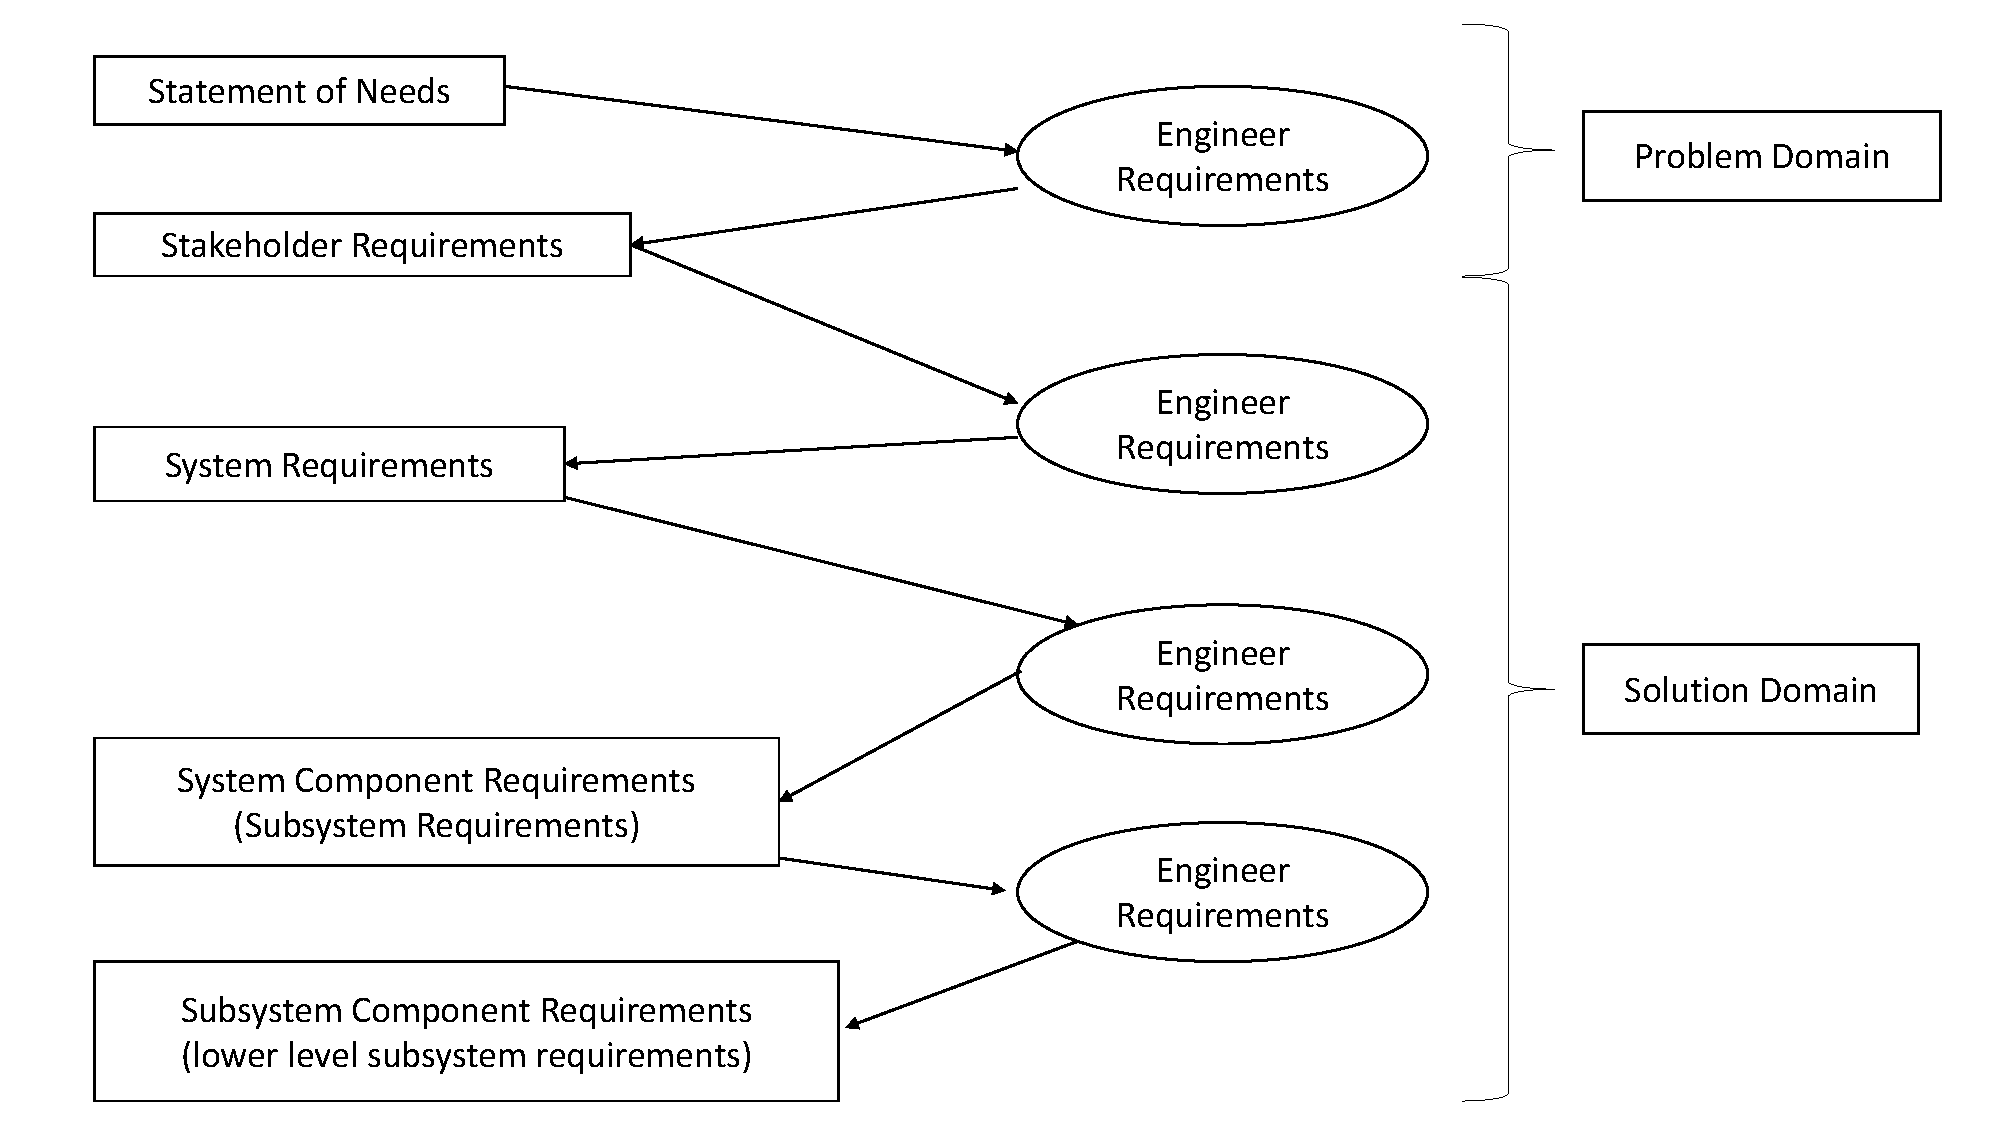
\includegraphics[scale=0.38]{img/levels-of-requirements-engineering.pdf}
	\caption{Entwicklungsprozess der Anforderungen}
	{\footnotesize \cite[Quelle: in Anlehnung an ][S.28]{hull_requirements_2011}}
	\label{abb:entwAnforderung}
	%		{\scriptsize \textit{Alle Rechte, einschließlich der Vervielfältigung, Veröffentlichung, Bearbeitung und Übersetzung bleiben der SV Informatik GmbH vorbehalten.}}
\end{figure}

Das \enquote{statement of needs} ist der Startpunkt für die Entwicklung einer Anforderung die am Ende des Prozesses, der in Abbildung \vref{abb:entwAnforderung} dargestellt ist, präzise dokumentiert sein wird. Dieses ist am Anfang immer ein Ausdruck eines Anspruchs oder Wunsches an das zu entwerfende System; dabei bildet das \enquote{statement} und die \enquote{stakeholder requirements} die \enquote{problem domain}. Diese definiert grundständige Methodik, wie auch eine nicht-technische Herangehensweise, die auf die Projektbeteiligten (\enquote{stakeholder}) angepasst ist. Nachfolgend werden die Projektbeteiligen als \enquote{stakeholder} bezeichnen, dabei ist die Rolle beschrieben als \enquote{(Stakeholder) sind Personen oder Organisationen, die ein potenzielles Interesse an einem zukünftigen System haben und somit in der Regel auch Anforderungen an das System stellen.}\autocite[][S.8]{partsch_requirements-engineering_2010} Später definiert die \enquote{problem domain} den Zweck des Systems -- dadurch ist bei der Ermittlung der Anforderungen die Frage \enquote{Was ist der Zweck des Systems?} anstelle \enquote{Was soll das System ihrer Meinung nach tun?}. Dies soll die \enquote{stakeholder} extrinsisch motivieren über den Zweck des zu entwerfenden Systems und nicht über einen möglichen Lösungsweg (das Wie) nachzudenken. Durch diesen Ansatz folgen Antworten nach dem Muster \enquote{Ich möchte etwas tun können ...} -- wissenschaftlich bzw. literarisch betrachtet sind diese Form der Anforderungen als \enquote{capability requirement(s)}\autocite[vgl.][S.94]{hull_requirements_2011} bekannt. Sie stellen die wichtigsten Erkenntnisse in der \enquote{problem domain} dar. Nun wird im weiteren Verlauf ein Modell konstruiert, das den Projektbeteiligten, den \enquote{stakeholder}, präsentiert wird. Dies unterliegt der Einschränkung, dass es jede/jedem Projektbeteiligte/n versteht. Denn sie validieren das konstruiert Modell in jedem weiteren Schritt, der in Abbildung \vref{abb:entwAnforderung}, ersichtlich ist. Die Anforderungen an das Modell sind quantitativ gering: es muss nicht-technisch sein und es muss geeignet sein die Anforderungen an das Systems abzubilden. Eine solche Darstellung ist dann geeignet, wenn sie den gewünschten Zweck an das System abbildet, das heißt, dass sie keine technischen Details zeigt, sondern einen Überblick bietet. Ein \enquote{use scenario}\autocite[vgl.][S.94]{hull_requirements_2011} wird meist verwendet, da es sich eignet menschliche Aktionen bzw. Ziele darzustellen. Abschließend müssen die \enquote{stakeholder}-Anforderungen folgende Kriterien erfüllen: 

\begin{itemize}
	\item kurz und prägnant formulierte Beschreibung, jedoch einfach zu verstehen und
	\item gleichzeitig sollten sie nicht-technisch aber realistisch formuliert sein.
\end{itemize}
 
 Die \enquote{solutions domain}, die auf Abbildung \vref{abb:entwAnforderung} zu sehen ist, ist die Nachfolgerin von der \enquote{problem domain}. Der Hauptunterschied zwischen den beiden Bereichen ist, dass die \enquote{solution domain} idealtypisch qualitativ hochwertig beschriebene Anforderungen als \enquote{Input} bekommt. Dazu konträr erhält die \enquote{problem domain} vage formulierte Wunschliste oder einem nicht klar definierten Ziel als initialen \enquote{Input}. Ausgehend von der Aussage von E. Hull, \enquote{in an ideal world, all the requirements would be clearly articulated, individual test able requirements}\autocite[][S.115]{hull_requirements_2011}, ist zu deduzieren, dass viele Ebenen zu erforschen gibt, um dieser Aufforderung zu entsprechen. So muss iterativ in jeder Ebene eine neue Analyse des \enquote{Inputs} erfolgen, um einen Ausgangspunkt für das weitere Vorgehen zu initialisieren. Die Komplexität diese Ebenen ist anhängig von dem Grad der Innovation sowie vom Kontext des zu entwickelnden Systems. Jede Entscheidung während des Prozess kann mögliche Entscheidungspfade in einer anderen Ebene verhindern. Ziel des Prozesses ist es, ein Anforderungsdokument/-katalog zu entwerfen, das laut der gesichteten Literatur in verschiedenen Repräsentationen vorliegen kann. Dennoch sollten primäre Bestandteile, wie die Rahmenbedingungen, die Projektbeteiligten, die Projektaspekte und die funktionale/nicht-funktionale Anforderungen, enthalten sein. Ein Beispiel dieses Katalogs ist im Anhang \vref{appendixAnforderung} zur Ansicht enthalten.
 
\subsection{Cloud Computing}

\subsection{Container}

\subsection{\enquote{Deployment}} \label{defDeployment}

\section{Ist-Analyse des jetzigen \enquote{Deployment}-Prozesses}

\section{Konzeption eines container-basierten, automatisierten \enquote{Deployments}}